\documentclass{article}
\usepackage{xcolor}
\newcommand{\red}{\color{red}}
\usepackage{tikz}
\usepackage[width=128mm]{geometry}
\pagestyle{empty}

\begin{document}

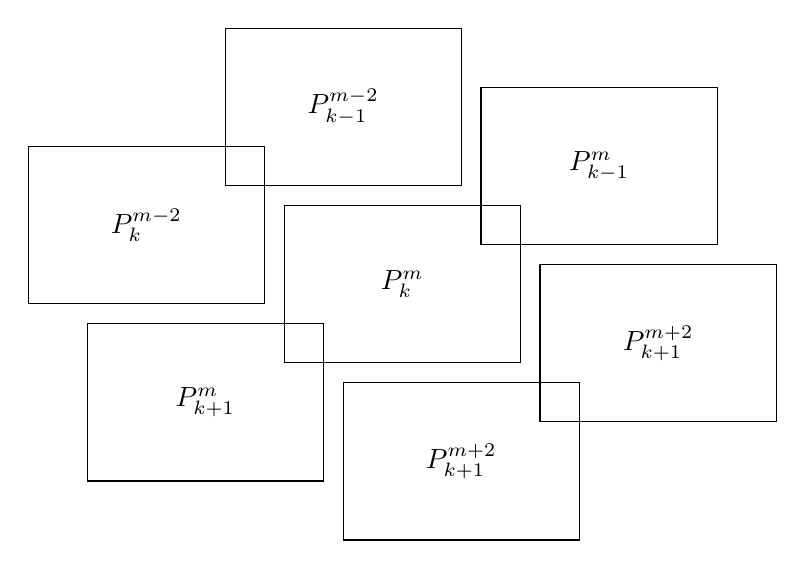
\begin{tikzpicture}
	\draw
	%% P column m-2
	(1.75,3.75) -- +(3,0) -- +(3,2) -- +(0,2) -- +(0,0) +(1.5,1) node{$P_{k-1}^{m-2}$}
	(-.75,2.25) -- +(3,0) -- +(3,2) -- +(0,2) -- +(0,0) +(1.5,1) node{$P_{k}^{m-2}$}

	%% P column m
	(5,3) -- +(3,0) -- +(3,2) -- +(0,2) -- +(0,0) +(1.5,1) node{$P_{k-1}^{m}$}
	(2.5,1.5) -- +(3,0) -- +(3,2) -- +(0,2) -- +(0,0) +(1.5,1) node{$P_{k}^{m}$}
	(0,0) -- +(3,0) -- +(3,2) -- +(0,2) -- +(0,0) +(1.5,1) node{$P_{k+1}^{m}$}

	%% P column m+2
	(5.75,.75) -- +(3,0) -- +(3,2) -- +(0,2) -- +(0,0) +(1.5,1) node{$P_{k+1}^{m+2}$}
	(3.25,-.75) -- +(3,0) -- +(3,2) -- +(0,2) -- +(0,0) +(1.5,1) node{$P_{k+1}^{m+2}$}

	;
\end{tikzpicture}

\end{document}
